\section{Convergencia de los tractogramas}
\label{sec:resultado_estabilidad}

El algoritmo \ref{alg:itract} de la secci\'on \ref{sec:convergencia} genera
tractogramas mediante un procedimiento Monte Carlo. Los tractogramas creados
de esta manera son inherentemente estoc\'asticos. Queremos analizar si dado
un n\'umero suficiente de part\'iculas el resultado del algoritmo converge.
Para ello utilizamos la t\'ecnica estad\'istica de $bootstrap$. Creamos una 
poblaci\'on de \textit{streamlines} y luego estudiamos como se comportan la
media y la varianza de los tractogramas. El proceso es el detallado en la
secci\'on \ref{sec:tractogramas}. Las Figuras \ref{fig:m1}, \ref{fig:m2} y 
\ref{fig:m3} muestran, para tres semillas distintas, cinco cortes coronales
del tractograma creado usando $15000$ \textit{streamlines}. Las figuras
\ref{fig:s1}, \ref{fig:s2} y \ref{fig:s3} muestran la varianza de cada
voxel dentro de un mismo corte coronal entre tractogramas creados con
distintas cantidades de submuestras. \\

La figura \ref{fig:mv} muestra la media y varianza de los voxels $A$, $B$ 
y $C$ marcados en las figuras \ref{fig:s1}, \ref{fig:s2} y \ref{fig:s3}.
Estos voxels fueron los que mayor varianza presentaron al generar
tractogramas usando subpoblaciones de $2000$ \textit{streamlines}.\\

\begin{figure}[h!]
   \centering
    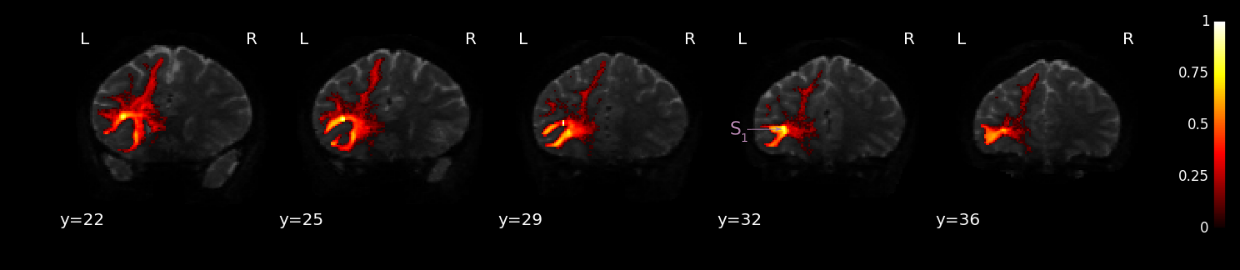
\includegraphics[width=\textwidth]{img/m1.png}
    \caption{Tractograma generado desde la semilla $S_1$ utilizando $15000$
             $streamlines$.}
    \label{fig:m1}
\end{figure}

\begin{figure}[h!]
   \centering
    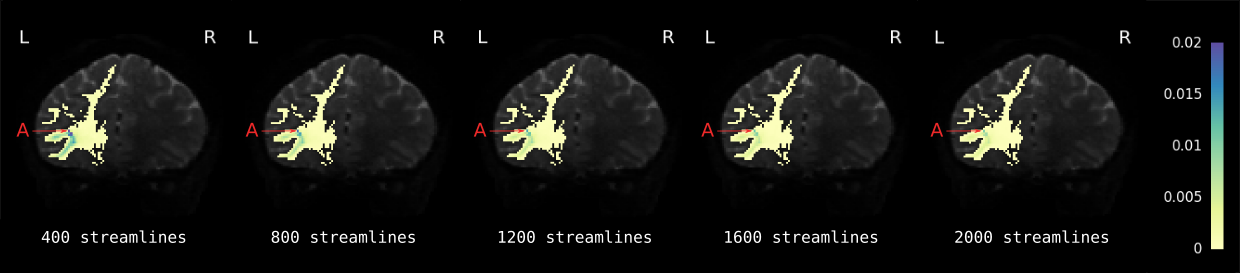
\includegraphics[width=\textwidth]{img/s1.png}
    \caption{Desviaci\'on est\'andar en un corte axial de los tractogramas
             de la semilla $S_1$ variando la cantidad de $streamlines$.}
    \label{fig:s1}
\end{figure}

\begin{figure}[h!]
   \centering
    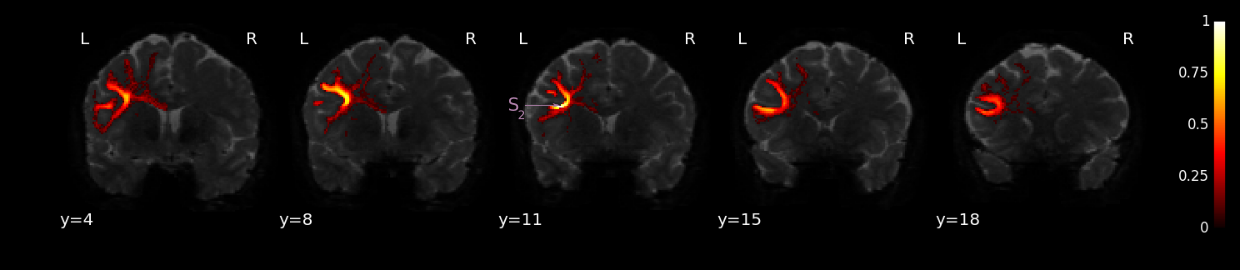
\includegraphics[width=\textwidth]{img/m2.png}
    \caption{Tractograma generado desde la semilla $S_2$ utilizando $15000$
             $streamlines$.}
    \label{fig:m2}
\end{figure}

\begin{figure}[h!]
   \centering
    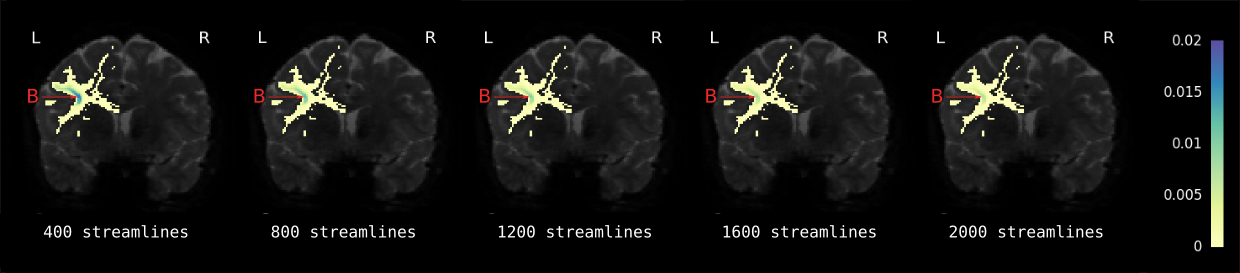
\includegraphics[width=\textwidth]{img/s2.png}
    \caption{Desviaci\'on est\'andar en un corte axial de los tractogramas
             de la semilla $S_2$ variando la cantidad de $streamlines$.}
    \label{fig:s2}
\end{figure}

\begin{figure}[h!]
   \centering
    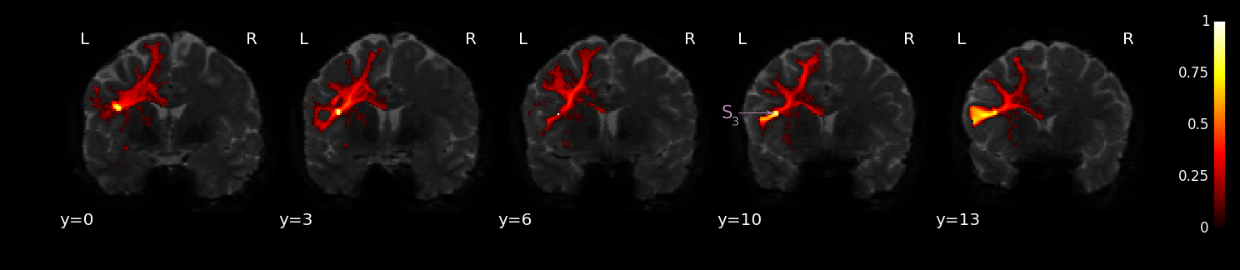
\includegraphics[width=\textwidth]{img/m3.png}
    \caption{Tractograma generado desde la semilla $S_3$ utilizando $15000$
             $streamlines$.}
    \label{fig:m3}
\end{figure}

\begin{figure}[h!]
   \centering
    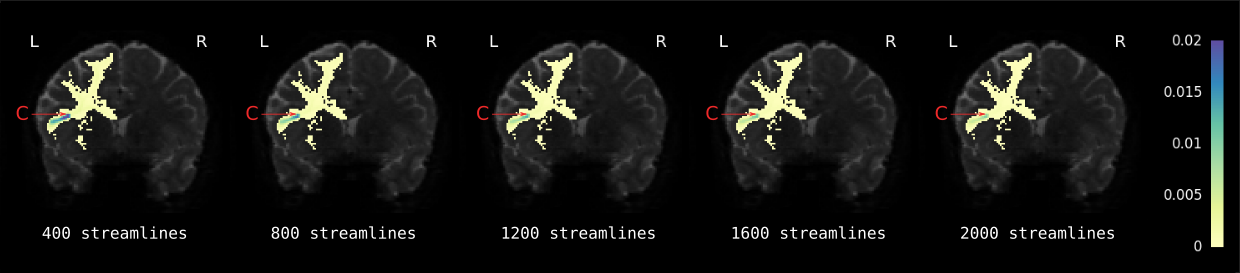
\includegraphics[width=\textwidth]{img/s3.png}
    \caption{Desviaci\'on est\'andar en un corte axial de los tractogramas
             de la semilla $S_3$ variando la cantidad de $streamlines$.}
    \label{fig:s3}
\end{figure}

\begin{figure}[h!]
   \centering
    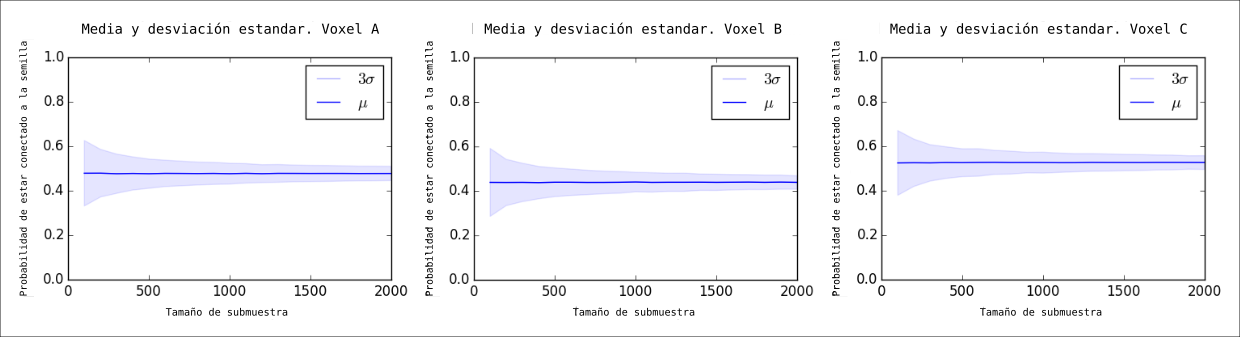
\includegraphics[width=\textwidth]{img/med_var_all.png}
    \caption{Media y desviaci\'on est\'andar de los voxels $A$, $B$ y $C$.
             Estos fueron los voxels con mayor varianza entre tractogramas
             generados con $2000$ $streamlines$.}
    \label{fig:mv}
\end{figure}
